\begin{frame}{Posing the Problem}
    % Introduce the Navier-Stokes Equations for incompressible flow

    \begin{block}{2D incompressible Navier-Stokes Eq.}
        Adimensionalizing the problem 
        \begin{align*}
          \frac{\partial \textbf{u}}{\partial t} + \textbf{u} \cdot \nabla \textbf{u} - \frac{1}{\Rey} \Delta \textbf{u} + \nabla p = 0 \label{eq:Ns_normalized} \\
          \nabla\cdot\vf{u} = 0 \notag
        \end{align*}
        with $\vf{u} = (u,v)$ the velocity field and $\Rey := \frac{\rho U L}{\mu}$ is the \textit{Reynolds number}.
    \end{block}


    \textbf{Boundary Conditions:}\\
    Incoming flow from the left side, between two walls and free on the right.
    \begin{align*}
        &\text{Left:}\quad & u &= 1,  & v &= 0, & \partial_{\vf{n}} p &= 0 \\
        &\text{Right:}\quad & \partial_{\vf{n}} u &= 0, & \partial_{\vf{n}} v &= 0, & p &= 0 \\
        &\text{Top and Bottom (Slip):}\quad & \partial_{\vf{n}} u &= 0, & v &= 0, & \partial_{\vf{n}} p &= 0
    \end{align*}



\end{frame}


\begin{frame}{Discretization and Boundary Conditions}
% Explaining treatment of boundary conditions and the body

\begin{columns}
    \begin{column}{0.5\textwidth}
        \textbf{Border of the Domain:}
        \begin{itemize}
            \item Domain discretization: Red for the domain, black dots for inner cells, blue for ghost cells.
            \item Boundary condition treatment: e.g., \(v_{0,j} = -v_{1,j}\) in ghost cells to set $v = 0$ on the left boundary.
        \end{itemize}

        \vspace{0.5cm}
        \textbf{Body:}
        \begin{itemize}
            \item The fluid is set to be at rest, simulating a no-slip boundary condition on the body's surface.
        \end{itemize}
    \end{column}
    \begin{column}{0.5\textwidth}
        \begin{figure}
            \centering
            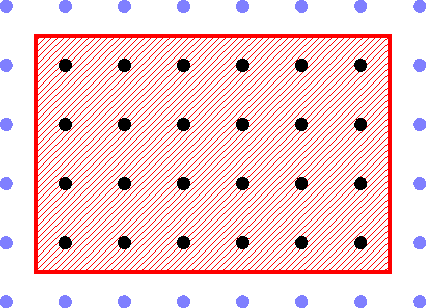
\includegraphics[width=0.7\linewidth]{graphics/grid.pdf}
            % Uncomment the next line if a caption is needed
            \caption{Grid representation with ghost cells.}
        \end{figure}
    \end{column}
\end{columns}

\end{frame}

\begin{frame}{Chorin's Splitting Method}
% Simplified overview of the method's steps for clarity and emphasis

\begin{block}{Overview}
Chorin's method simplifies the Navier-Stokes equations into sequential steps, enhancing numerical stability and computational efficiency (\cite{Chorin1967NumericalNS,Boyd2001ChebyshevFourier}).
\end{block}

\textbf{Steps:}
\begin{enumerate}
    \item Advection: $\displaystyle\frac{\vf{u}^a - \vf{u}^n}{\Delta t} + \vf{u}^n\cdot\nabla\vf{u}^n = 0$
    \item Diffusion: $\displaystyle\frac{\vf{u}^* - \vf{u}^a}{\Delta t} = \frac{1}{\mathrm{Re}}\laplacian\vf{u}^n$
    \item Pressure: $\displaystyle\laplacian p^{n+1} = \frac{1}{\Delta t}\nabla\cdot\vf{u}^*$
    \item Velocity correction: $\displaystyle\vf{u}^{n+1} = \vf{u}^* - \Delta t\nabla p^{n+1}$
\end{enumerate}

\end{frame}

\begin{frame}{1st Step: Semi-Lagrangian method}
  Solving the advection equation with velocity $\vf{u}$:
  \begin{equation*}
    \frac{\mathrm{D}\vf\psi}{\mathrm{D}t}=\frac{\partial \vf{\psi}}{\partial t} + \vf{u}\cdot\nabla\vf{\psi} = 0
  \end{equation*}
  Discretization of the material derivative:

  \begin{equation*}
    \frac{\vf{\psi}(\vf{x}_{i,j}, t^{n+1}) - \vf{\psi}(\vf{x}_{i,j} - \Delta t\vf{u}(\vf{x}_{i,j}, t^n), t^n)}{\Delta t} = 0
  \end{equation*}
  \begin{figure}
    \centering
    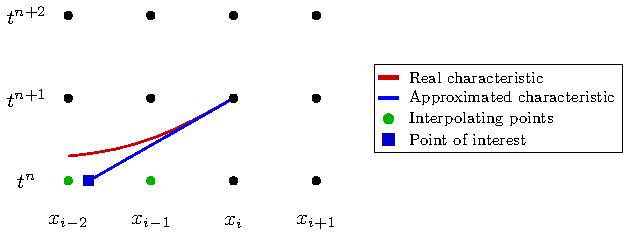
\includegraphics[width=0.8\textwidth]{graphics/characteristics.pdf}
  \end{figure}
\end{frame}

% \begin{frame}{2. Step: Adding diffusion}
%     %Maybe having this much slides is a bit over the top but just to showcase the idea
% \end{frame}


\begin{frame}{3rd Step: Solving the Poisson Equation for Pressure}
%draft
    \textbf{Approach:}
    \begin{itemize}
        \item \text{Laplacian approximation:} Employ a 5-point stencil with finite difference method.
        \item \text{Matrix representation:} Formulate as $\vf{A}\vf{p}=\vf{f}$.
    \end{itemize}
    
    \textbf{Solution via Cholesky decomposition:}
    \begin{itemize}
        \item Transform \(\vf{A}\) for positive definiteness: \(-\vf{A}\vf{p} = -\vf{f}\).
        \item Cholesky decomposition: Efficiently solves for \(\vf{p}\) .
        \item Stability and speed in solving \(\vf{A}\vf{p}=\vf{f}\), critical for fluid dynamics simulations.
    \end{itemize}
    
%Maybe we can include here a graphic which we can use to show how thos method works...
\end{frame}


% \begin{frame}{4. Step: }



%     % I would say that just if it suits and looks nice, too much formulas for saying it is basically the equation we present before wouldnt be necessary
% %  \begin{minipage}{0.2\textwidth}
% %    $$
% %      \implies
% %    $$
% %  \end{minipage}\hspace{-1cm}
% %  \begin{minipage}{0.79\textwidth}
% %    \begin{align*}
% %      \frac{\vf{u}^{n+1} - \vf{u}^n}{\Delta t} + \vf{u}^n\cdot\nabla\vf{u}^n & = -\nabla p^{n+1} + \frac{1}{\Rey}\laplacian\vf{u}^n \\
% %      \nabla\cdot\vf{u}^{n+1}                                                & = 0
% %    \end{align*}
% %  \end{minipage}
% \end{frame}